\section{Discussion}

For logistic regression, the following figure is gotten from 
article ~\cite{ComparisonData}. 

\begin{figure}[H]
\begin{center}
    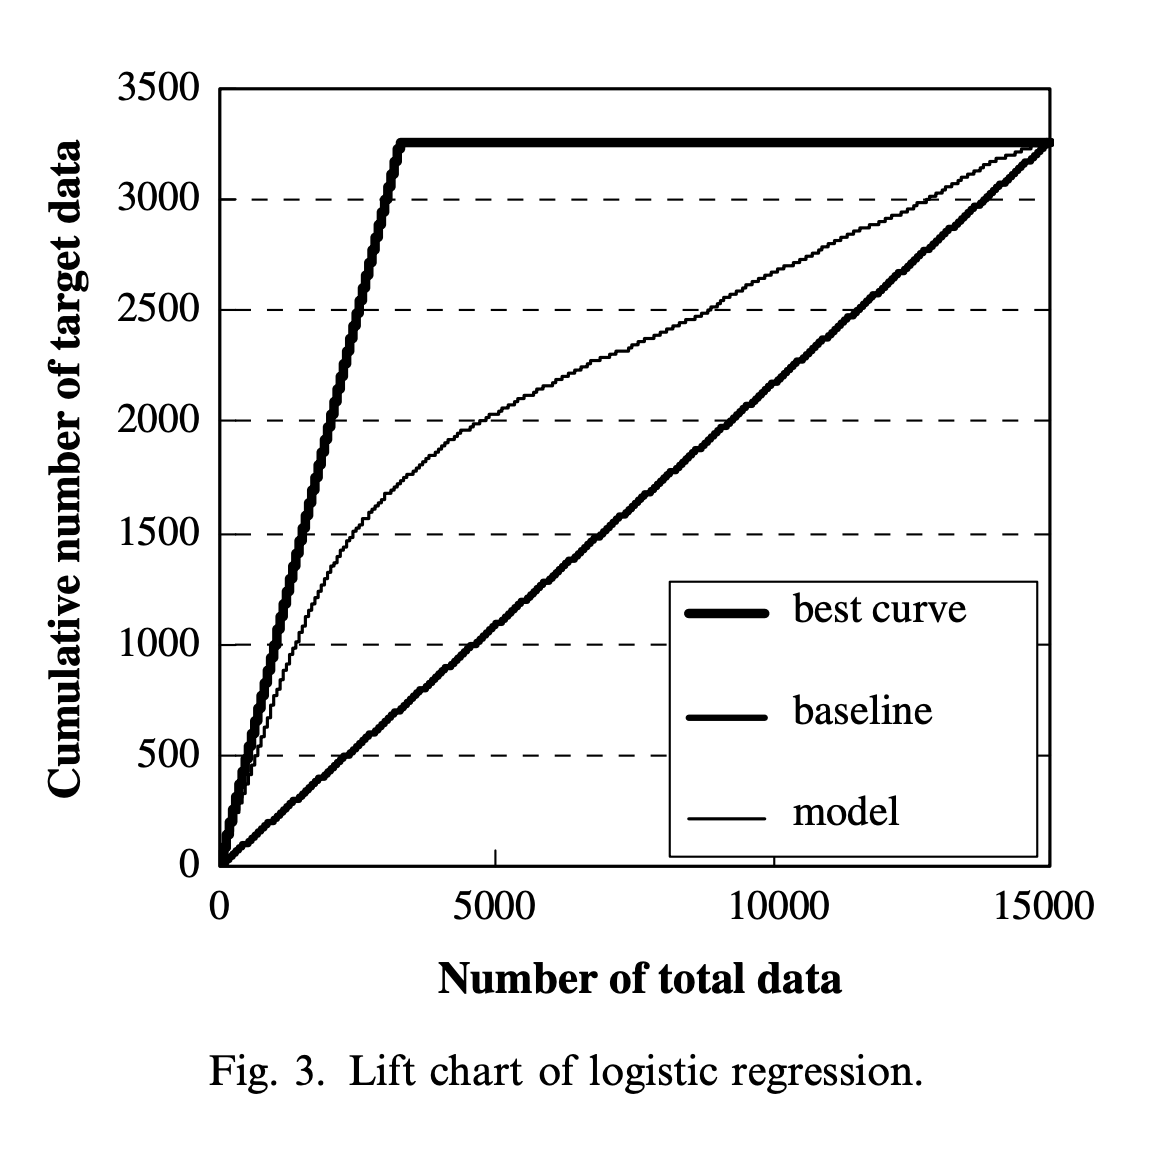
\includegraphics[width=0.75\textwidth, height=0.5\textheight]{figures/logistic_article.png}
\end{center}
\caption[caption]{Figure 3 from relating article ~\cite{ComparisonData}}
\end{figure}

Comparing this figure to figure ~\ref{fig:logistic1} in our 
results shows that the logistic method we have used on the 
dataset gives very similar results to the article, as expected. 

From figure ~\ref{fig{logistic3}}, we see that we get 
better results using random oversampling (and balanced weighting?). 

